%%%%%%%%%%%%%%%%%%%%%%%%%%%%%%%%%%%%%%%%%
% Short Sectioned Assignment
% LaTeX Template
% Version 1.0 (5/5/12)
%
% This template has been downloaded from:
% http://www.LaTeXTemplates.com
%
% Original author:
% Frits Wenneker (http://www.howtotex.com)
%
% License:
% CC BY-NC-SA 3.0 (http://creativecommons.org/licenses/by-nc-sa/3.0/)
%
%%%%%%%%%%%%%%%%%%%%%%%%%%%%%%%%%%%%%%%%%

%----------------------------------------------------------------------------------------
%	PACKAGES AND OTHER DOCUMENT CONFIGURATIONS
%----------------------------------------------------------------------------------------

\documentclass[paper=a4, fontsize=11pt]{scrartcl} % A4 paper and 11pt font size 

\usepackage[T1]{fontenc} % Use 8-bit encoding that has 256 glyphs
\usepackage[english]{babel} % English language/hyphenation
\usepackage{amsmath,amsfonts,amsthm} % Math packages

\usepackage{sectsty} % Allows customizing section commands
%\allsectionsfont{\centering \normalfont\scshape} % Make all sections centered, the default font and small caps

\usepackage{fancyhdr} % Custom headers and footers
\pagestyle{fancyplain} % Makes all pages in the document conform to the custom headers and footers
\fancyhead{} % No page header - if you want one, create it in the same way as the footers below
\fancyfoot[L]{} % Empty left footer
\fancyfoot[C]{} % Empty center footer
\fancyfoot[R]{\thepage} % Page numbering for right footer
\renewcommand{\headrulewidth}{0pt} % Remove header underlines
\renewcommand{\footrulewidth}{0pt} % Remove footer underlines
\setlength{\headheight}{13.6pt} % Customize the height of the header

\numberwithin{equation}{section} % Number equations within sections (i.e. 1.1, 1.2, 2.1, 2.2 instead of 1, 2, 3, 4)
\numberwithin{figure}{section} % Number figures within sections (i.e. 1.1, 1.2, 2.1, 2.2 instead of 1, 2, 3, 4)
\numberwithin{table}{section} % Number tables within sections (i.e. 1.1, 1.2, 2.1, 2.2 instead of 1, 2, 3, 4)

\setlength\parindent{0pt} % Removes all indentation from paragraphs - comment this line for an assignment with lots of text

\usepackage{bbm}
\usepackage{graphicx}
\usepackage{xcolor} % For color
\usepackage{subcaption}
\usepackage{booktabs}

\usepackage{tikz} % For graphs
\usetikzlibrary{positioning}
\usetikzlibrary{calc}

\usepackage{enumerate} % For lettered enumeration

\usepackage{algorithm}
%\usepackage{algorithmic}
\usepackage[noend]{algpseudocode} % for pseudocode

%----------------------------------------------------------------------------------------
%	TITLE SECTION
%----------------------------------------------------------------------------------------

\newcommand{\horrule}[1]{\rule{\linewidth}{#1}} % Create horizontal rule command with 1 argument of height

\title{	
\normalfont \normalsize 
\horrule{0.5pt} \\[0.4cm] % Thin top horizontal rule
\huge Assignment Five \\ % The assignment title
\horrule{2pt} \\[0.5cm] % Thick bottom horizontal rule
}

\author{
	Matthew C.~Scicluna\\
	D\'epartement d'Informatique et de Recherche Op\'erationnelle\\
	Universit\'e de Montr\'eal\\
	Montr\'eal, QC H3T 1J4 \\
	\texttt{matthew.scicluna@umontreal.ca}
}


\date{\normalsize\today} % Today's date or a custom date

\begin{document}

\maketitle % Print the title

%----------------------------------------------------------------------------------------
%	PROBLEM 1
%----------------------------------------------------------------------------------------

\section{Importance Sampling}
We estimate the normalizing constant $Z_p$ for an un-normalized Gaussian
$\tilde{p}̃(x) = \exp\left(-\frac{1}{2\sigma_p^2} x^2\right)$; i.e. we have $p(\cdot)\sim N(0,\sigma_p^2)$ with $p(x) = \tilde{p}̃(x)/Z_p$ . Given N i.i.d. samples $x^{(1)} , \cdots , x^{(N)}$ from a standard normal $q(\cdot) \sim N (0, 1)$, we consider the following importance sampling estimate $\hat{Z} = \frac{1}{N}\sum_{i=1}^N \frac{\tilde{p}̃(x^{(i)})}{q(x^{(i)})}$. 

\begin{enumerate}[(a)]
	\item We can see this estimator is unbiased since:
	\begin{align}
	\mathbb{E}_{X\sim q}\left\{\hat{Z}\right\}&=\mathbb{E}_{X\sim q}\left\{ \frac{1}{N}\sum_{i=1}^N \frac{\tilde{p}̃(X^{(i)})}{q(X^{(i)})} \right\} \\
	&=\frac{1}{N}\sum_{i=1}^N \mathbb{E}_{X\sim q}\left\{ \frac{\tilde{p}̃(X^{(i)})}{q(X^{(i)})} \right\} \\
	&= \int_X \frac{\tilde{p}̃(X)}{q(X)}q(X)dX \\
	&= Z_p
	\end{align}
	where (1.4) follows from $\int \tilde{p}̃ = Z_p$
	\item Let $f(X)=\frac{\tilde{p}̃(X)}{q(X)}$ Then $Var(\hat{Z})$ can be easily computed
	\begin{align}
	Var(\hat{Z}) &= Var\left\{\frac{1}{N}\sum_{i=1}^N \frac{\tilde{p}̃(X^{(i)})}{q(X^{(i)})}\right\}\\
	&= \frac{1}{N^2}\sum_{i=1}^N Var \left\{\frac{\tilde{p}̃(X^{(i)})}{q(X^{(i)})}\right\}\\
	&=\frac{1}{N}Var(f(X))
	\end{align}
	Provided that $Var(f(X))$ is finite
	\item To find the values of $\sigma^2_p$ which make $Var(f(X))$ finite, it is enough to find the values which make $\mathbb{E}(f^2)$ finite.
	\begin{align}
	\mathbb{E}(f(X)^2) &= \int_X \frac{\tilde{p}̃(X)^2}{q(X)}dX\\
	&= \int_X \sqrt{2\pi}\frac{\exp\left(-\frac{1}{2\sigma_p^2} X^2\right)^2}{\exp\left(-\frac{1}{2} X^2\right)} dX \\
	&= \sqrt{2\pi}\int_X\exp\left(-\frac{X^2}{2\sigma_c^2}\right) dX
	\end{align}
	Where $\sigma_c^2=\frac{\sigma_p^2}{2-\sigma_p^2}$. There are three cases. If $\sigma_c^2<0$ then the integral clearly diverges. If $\sigma_c^2=0$ it is undefined. If $\sigma_c^2>0$ then (1.10) is an unnormalized Gaussian, and so:
	\begin{align}
	\mathbb{E}(f(X)^2) &= 2\pi\sigma_c \\
	&= \begin{cases}2\pi\sqrt{\frac{\sigma_p^2}{2-\sigma_p^2}} & \text{for } 0 < \sigma_p^2 < 2\\
	\infty & \text{o.w.}
	\end{cases}
	\end{align}
\end{enumerate}

\section{Gibbs Sampling and Mean Field Variational Inference}

We consider the Ising model with binary variables $X_s\in\{0,1\}$ and a factorization of the form:
\begin{equation}
p(x;\eta)=\frac{1}{Z_p}\exp\left( \sum_{s\in V} \eta_s x_s + \sum_{\{s,t\}\in E} \eta_{st} x_s x_t \right)
\end{equation}

On the $7\times7$ 2D toroidal grid

\begin{enumerate}[(a)]
	\item We derive the Gibbs sampling updates for this model. The algorithm is detailed in Algorithm 1:
	\begin{algorithm} % enter the algorithm environment
		\caption{Calculate $\mu_s = p(X_s = 1)$ using Gibbs Sampling} % caption
		\label{alg1} % and a label for \ref{} commands later in the document
		\begin{algorithmic}[1] % enter the algorithmic environment
			\For{states $i,j \in \{1, \cdots, 49\}$ and $\{i,j\}\in E$}
			\State{$\eta_i \leftarrow (−1)^i$}
			\Comment{Initialize Nodes as per HW}
			\State{$ \eta_{i,j} \leftarrow 0.5$}
			\Comment{Initialize Edges as per HW}
			\State Sample {$x_{i}^{(0)} \sim Bern(0.5)$}
			\Comment{Initialize variables randomly}
			\EndFor
			\For{Epoch $t \in \{0,\cdots, 5999\}$}
			\For{$i \in \{1, \cdots, 49\}$}
			\State Sample \(x_i^{(t+1)} \sim p\left(x_i = 1 \mid x_1^{(t+1)},\cdots, x_{i-1}^{(t+1)}, x_{i+1}^{(t)},\cdots,x_{49}^{(t)}\right)\)
			\EndFor
			\EndFor
			\For{$i \in \{1, \cdots, 49\}$}
			\State $\mu_i \leftarrow \frac{1}{5000}\sum_{t=1001}^{6000}x_i^{(t)}$
			\Comment{Compute Monte Carlo estimates of Moments}
			\EndFor
			\Return $\mu_1, \cdots, \mu_{49}$
		\end{algorithmic}
	\end{algorithm}
	
	To compute $p(x_i = 1 \mid x_{\neg i})$, we notice that it is enough to compute the odds ratio since:
		\begin{align}
		p(x_i = 1 \mid x_{\neg i}) &= \frac{p(x_i = 1, x_{\neg i})}{\sum_{k=0}^{1}p(x_i = k, x_{\neg i})}\\
		&= \frac{1}{1 + \frac{p(x_i = 0, x_{\neg i})}{p(x_i = 1, x_{\neg i})}}\\
		&= \frac{1}{1+\exp(-Z)}\\
		&= \sigma\left(Z\right)
		\end{align}
	Where $Z=log \frac{p(x_i = 1, x_{\neg i})}{p(x_i = 0, x_{\neg i})}$. 
	We compute the log joint density with $x_i=1$ and $x_i=0$
	\begin{align}
		log p(x_i = 1, x_{\neg i}) &=\sum_{s\in V} \eta_s x_s + \sum_{\{s,t\}\in E} \eta_{st} x_s x_t\\
		&=\eta_i + \sum_{j \ne i}\eta_j x_j + \sum_{j\in N(i)} \eta_{ij} x_j + \sum_{\substack{j\not\in N(i) \\ \{k,j\}\in E}} \eta_{kj}x_kx_j\\
		&= \eta_i + \sum_{j\in N(i)} \eta_{ij} x_j + C\\
		log p(x_i = 0, x_{\neg i}) &= \sum_{j \ne i}\eta_j x_j + \sum_{\substack{j\not\in N(i) \\ \{k,j\}\in E}} \eta_{kj}x_kx_j\\
		&=C
	\end{align}
	And so subbing (2.8) and (2.10) into $Z$ gives us
	\begin{align}
	Z = \eta_i + \sum_{j\in N(i)} \eta_{ij} x_j
	\end{align}
	Hence $p(x_i = 1 \mid x_{\neg i}) = \sigma\left(\eta_i + \sum_{j\in N(i)} \eta_{ij} x_j\right)$
	
	Ran the experiment 10 times and computed the estimated moments. We found that the standard deviations were very low, ranging from $0.002$ to $0.009$. The values are available in the code.
	
	
	\item We derive the naive mean field updates. Let $q(X_s=1) = \tau_s$
	We wish to do cyclic coordinate descent on $KL(q||p)$. Note that:
	\begin{align}
	KL(q||p) &= \mathbb{E}_q\{\log q(x)-\log p(x) \}\\
	&= \mathbb{E}_q\{\log q(x)\} - \mathbb{E}_q\{\log p(x)\}\\
	&= - H(q) -  \sum_{s\in V} \eta_s \mathbb{E}_q\{x_s\} - \sum_{\{s,t\}\in E} \eta_{st} \mathbb{E}_q\{x_s x_t\} + log(Z_p)\\
	&= - H(q) -  \sum_{s\in V} \eta_s \tau_s - \sum_{\{s,t\}\in E} \eta_{st} \tau_s\tau_t + log(Z_p)
	\end{align}
	Where (2.14) comes from (2.1) and using the mean field assumption.	For the update we compute the derivative. First we compute the derivative of $H(q)$
	\begin{align}
	\frac{\partial H(q)}{\partial \tau_s} &= \frac{\partial}{\partial \tau_s}\sum_{i}\mathbb{E}_q\{ \log q(x_i) \}\\
	&= \frac{\partial}{\partial \tau_s}\mathbb{E}_q\{ \log q(x_s) \}\\
	&= \frac{\partial}{\partial \tau_s}q(x_s)\log q(x_s) + (1-q(x_s))\log (1 - q(x_s))\\
	&= \frac{\partial}{\partial \tau_s}\tau_s\log \tau_s + (1-\tau_s)\log (1 - \tau_s)\\
	&= \log\left(\frac{\tau_s}{1-\tau_s}\right)
	\end{align}
	The rest of the derivative is easy:
	\begin{align}
	\frac{\partial KL(q||p)}{\partial \tau_s} &= \eta_s + \sum_{t\in N(s)} \eta_{st} \tau_t - \log\left(\frac{\tau_s}{1-\tau_s}\right) = 0\\
	&\Rightarrow \tau_s = \sigma\left( \eta_s + \sum_{t \in N(s)} \eta_{st} \tau_t \right)
	\end{align}
	We can derive the expression for $KL(q||p) - log(Z_p)$ using (2.15)
	\begin{align}
	&KL(q||p) - log(Z_p) = - H(q) -  \sum_{s\in V} \eta_s \tau_s - \sum_{\{s,t\}\in E} \eta_{st} \tau_s\tau_t\\
	&= -\sum_{s\in V} \eta_s \tau_s - \sum_{\{s,t\}\in E} \eta_{st} \tau_s\tau_t - \sum_{s}^{}\left(\tau_s\log \tau_s + (1-\tau_s)\log (1 - \tau_s)\right)
	\end{align}
	
	We did cyclic coordinate descent on $KL(q||p)$, sequentially updating each $\tau_s$. We monitored $KL(q||p) - log(Z_p)$ and plotted it per epoch in figure 2.1.
	
	\begin{figure}
		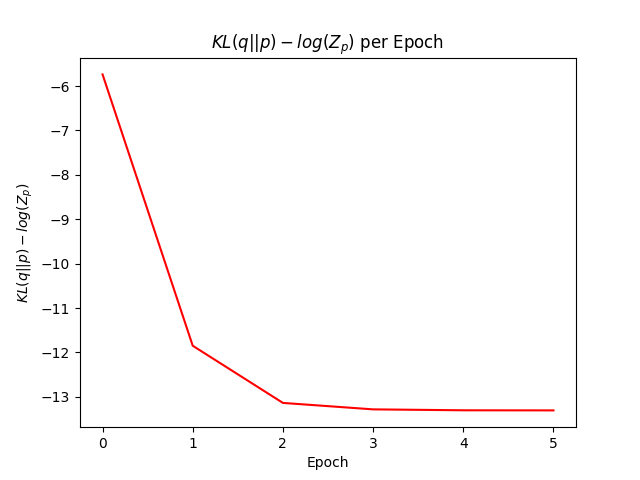
\includegraphics[width=.9\linewidth]{per_epoch.png}
		\caption{$KL(q||p) - log(Z_p)$ computed per epoch}
	\end{figure}
	
	We computed the $l_1$ distance between $\tau_s$ and $\mu_s$. We found that it was only $0.0077$. In this sense it was a good approximation. We tried several different initializations but found that the model did not get stuck in different local minima, and converged to the same parameters each time.
	
\end{enumerate}

\end{document}